\chapter{Proposed Scheme}\markright{Chapter 4: Proposed Scheme}\label{sec:proposed_scheme}

\section{Idea}
Our goal is to design the defense scheme against each evasive technique on different targets, GSI and BD, to achive the practical CNN based IoT malware detection on IoT devices.
In order to accomplish our goal, we propose an evasion-resilient IoT malware detection scheme with invalidating adversarial byte sequences and 1D convolutional filters.  
The main idea of our scheme is that there still remain regions which contribute to decision making in both manipulated targets after the attacks.
We aim to improve the detection accuracy by statically extracting/enhancing each valuable region of the target to the CNN model.

図 shows the manipulated area by adversaries and the area which have high degree of contribution for CNN to make decision on representative manipulated target.
The red area in each target is the area which has been manipulated.
In the case of AM, noise is added to the pixels, and in that of OM, the original BD is compressed or new code is inserted in these regions.
On the other hand, the yellow area is where contributes to decision making still remaining after the attack.
In the case of AM, it is the pixel region where noise cannot be added, and in that of OM, it is the byte sequence region which remain discretely after the compression.

In each defense scheme, the detection accuracy can be improved by feeding those yellow region effectively to the CNN model.
The representative schemes are explained in the following sections.

\section{Defense scheme against AM}
A defense scheme against AM, which is a malware whose GSI is manipulated, is explained in this section.

We focus on the fact that the adversary can manipulate only the pixels which match the BD whose information is unnecessary at runtime.
This is because the AM must maintain the original functionality of the malware even after the noise is added by the adversary.
In our proposal, we call these pixels Junk Pixels (JPs), and we think it would be possible to remove the noise by converting their pixel values into 0, which means turning them black pixels.

The two GSIs as shown in 図 are the AM GSI with noise added by adversary and the that with denoising for JPs in our proposal.
The red box area is the area where the pixel values are converted into 0 as JPs.
This pixel region corresponds to the byte sequences which contain unnecessary information at runtime, such as metadata and debugging information used while linking.
Thus, they can be regarded as pixels where the noise which contribute to benign decision can be added when AMs are created.

On the other hand, yellow box area is the area with no manipulation in our proposal.
This pixel area corresponds to the byte sequences that represents the malware behaviour and the data held.
Thus, it is judged to hold valuable information for the classification since it is difficult to manipulate these byte sequences affecting the malware function for adversary without any destructions.
Hence, we utilize JPs, which locate in this area, for our detection as it is.

By doing this denoising process, the detection without being misled by AMs would be possible since only the pixels which tend to be not manipulated can be used for our classification.


\section{Defense scheme against OM}
A defense scheme against OM, which is a malware whose BD is obfuscated with packing tools, is explained in this section.

In this defense scheme, we focus on the fact that the appearing order of discrete byte sequences remaining after obfuscation is invariant before and after packing.
Thus, showing the honrizontal connection of the byte sequences derived from the original BD can result in emphancizing valuable region remaining in OM for the CNN model.
We realize it by convoluting the GSI pixels in the horizontal direction with 1D filters.

I explain the method of convolution in the horizontal direction of pixels with a 1D filter, comparing with that in two dimentions with a 2D filter in the previous scheme.
図 shows the flow of the previous method using 2D convolutional filters, such as this blue flame, which are commonly used in image analysis due to correlation in both horizontal and vertical directions.
The figure with 6*6 squares in 図 represents the GSI, and each of them is a representaion of a pixel.
In particular, the yellow pixels represent pixels valuable information and the gray pixels represent pixels which are not necessary for classification due to tool-dependency.
Unlike common images, the correlation in the vertical direction is weak in GSIs since they are converted from byte sequences.
Furthermore, by convoluting with such 2D filters, both pixels, yellow ones and gray ones, coexist in the same filter especially in the convolution of the boundary of those pixel regions.
It can result in the false classification since the weight of valuable pixels in the decision becomes small in consequence of the useless pixels coexisting in the same filter.

On the other hand, in our proposal, the GSI is convoluted using 1D filters with a horizontal length as shown in the red frame in 図, which represents the flow of the proposal method.
In our proposal, we can emphasize the byte regions which are valuable for classification by showing the correlation of the appearing order of discrete byte sequences remaining after obfuscation to the CNN model.
Furthermore, it is possible to avoid the degradation of valuable pixel weight by the pixel which has coexisted in the vertical direction in the previous method at the boundary of both pixels.

As described above, by using 1D filters to show the horizontal correlations between encrypted byte sequences, we can improve the detection accuracy by highlighting features retained in the OM which are valuable for training CNN model even under the static analysis.

As shown in \figurename~\ref{fig:ssl_inspection}, there exists the difference of the percentage of communication with DV servers between benign apps and malwares.
\begin{figure}[p]
	\centering
	\hspace{-55pt}
	% \includegraphics[scale=0.34]{./figure/dv_unknown_inspection.pdf}
	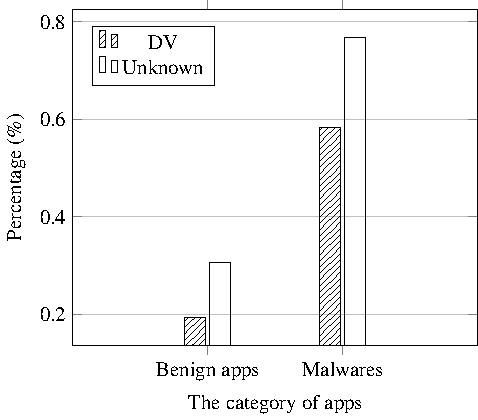
\includegraphics[scale=1.0, bb=9 9 200 200]{./figures/dv_unknown_inspection_tikz.pdf}
	% \includegraphics[scale=0.34]{./figure/ssl_inspection.pdf}
	\caption{The result of inspection regarding SSL server certificate} 
	\label{fig:ssl_inspection}
\end{figure}
\afterpage{\clearpage}
\newpage

